\documentclass{article}
\usepackage{ctex}
\usepackage{amsmath, amssymb}
\usepackage{booktabs}
\usepackage{geometry}
\geometry{a4paper, margin=1in}
\usepackage{titling}
\setlength{\droptitle}{50ex}
\pretitle{\begin{flushleft}\Large\bfseries}
\posttitle{\par\end{flushleft}}
\preauthor{\begin{flushleft}\fangsong}
\postauthor{\end{flushleft}}
\predate{\begin{flushleft}}
\postdate{\end{flushleft}}
\usepackage{etoolbox}
\patchcmd{\thebibliography}{\section*{\refname}}{}{}{}

\usepackage[utf8]{inputenc}
\usepackage[TS1,T1]{fontenc}
\usepackage{fourier, heuristica}
\usepackage{array, booktabs}
\usepackage{graphicx}
\usepackage[x11names]{xcolor}
\usepackage{colortbl}
\usepackage{caption}
\DeclareCaptionFont{blue}{\color{LightSteelBlue3}}

\newcommand{\foo}{\color{black}\makebox[0pt]{\textbullet}\hskip-0.5pt\vrule width 1pt\hspace{\labelsep}}

\newcommand{\upcite}[1]{\textsuperscript{\textsuperscript{\cite{#1}}}}

\usepackage{hyperref}
\hypersetup{hypertex=true,
            colorlinks=true,
            linkcolor=magenta,
            anchorcolor=magenta,
            citecolor=magenta}

\usepackage{background}
%\usepackage{amsrefs}

\title{《不定方程相关理论及其应用》开题报告}
\author{应数2101·郑欢誉·2214414387}
\date{\today}

\begin{document}

\maketitle
\thispagestyle{empty}
\backgroundsetup{scale = 1, angle = 0, opacity = 0.1,
  contents = {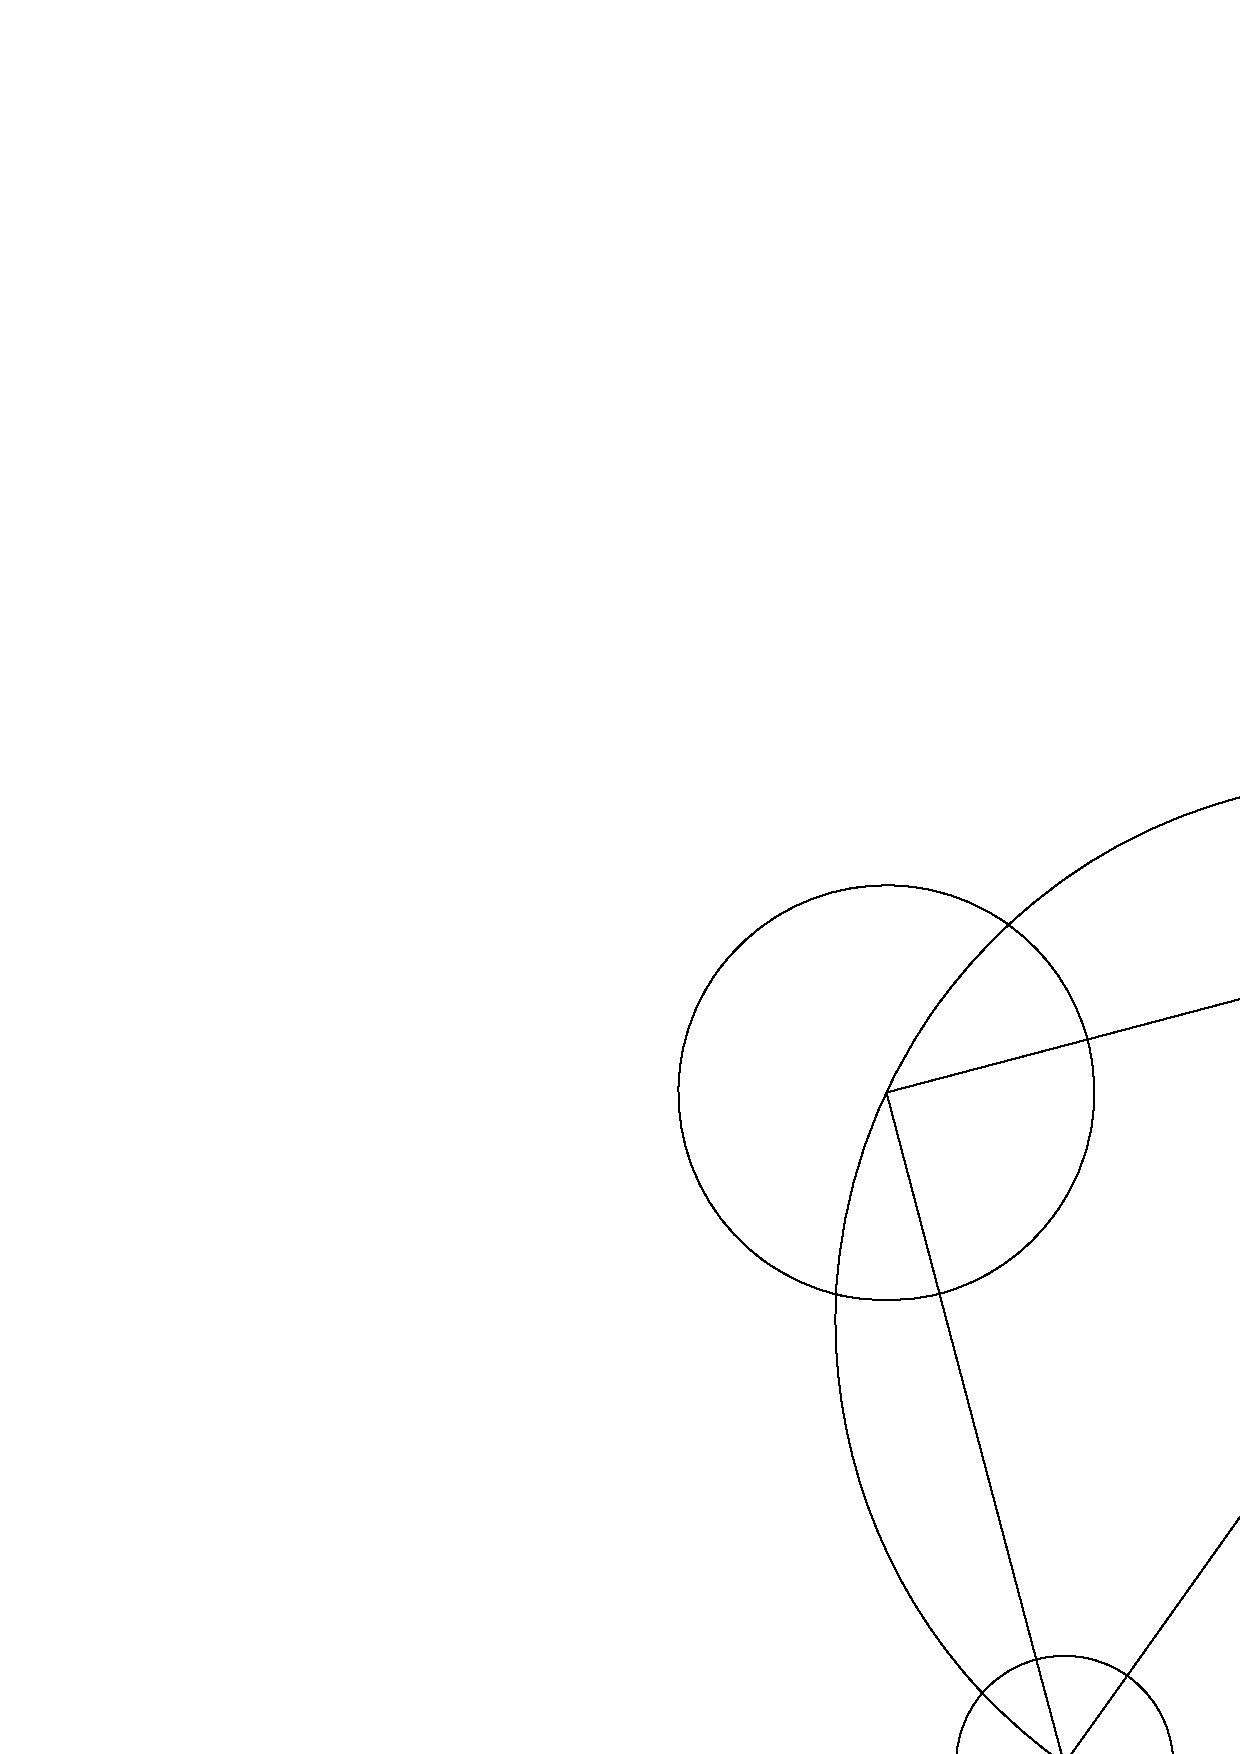
\includegraphics[width = \paperwidth,
  height = \paperheight, keepaspectratio]
  {bg.pdf}}}
  % Adjust filename and path to match your own image 
\newpage
\hrule

\part{研究背景和意义}

\noindent
不定方程,又称丢番图方程(Diophantine equation),是数学中研究整数解的多项式方程。它们得名于古希腊数学家Diophantus,他在著作《算术(Arithmetica)》中提出了一系列关于求解整数方程的问题。不定方程理论作为数论的一个重要分支,涉及许多经典问题,其中包括费马大定理(Fermat's Last Theorem)。\\

\noindent
在《算术》的问题II.8中,Diophantus提问:“如何寻找有理数$k,u,v$使得$k^2=u^2+v^2$”?他随后给出了$k=4$时的构造。1637年,法国数学家Pierre de Fermat在他的《算术》一书上这一问题旁的空白处写下了数学史上最著名的注释:

\begin{quote}
Cubum autem in duos cubos, aut quadratoquadratum in duos quadratoquadratos \& generaliter nullam in infinitum ultra quadratum potestatem in duos eiusdem nominis fas est dividere cuius rei demonstrationem mirabilem sane detexi. Hanc marginis exiguitas non caperet. 

然而,立方数不能分成两个立方数,4次方数不能分成2个4次方数,一般来说,任何高于平方的幂都不能分成两个同名幂。我确实发现了一种非常奇妙的证明,但因篇幅所限,无法写在书页的边缘。
\end{quote}

\noindent
Fermat的原始手稿已经遗失,但在此之前他的儿子Samuel将所有他在书页边缘写下的笔记集结出版,后人才得以知晓这一故事。实际上Fermat利用无穷递降法完整证明了幂次为4的情况,并于1670年发表。但并没有关于其它情况的证明留存下来,因此这一简单的陈述成为了数学史上最著名的未解之谜之一,吸引了数百年来无数数学家的研究。\\

\noindent
在接下来的几个世纪里,费马大定理的部分特例逐步得到验证。18世纪,Leonhard Euler证明了当幂次为3时的情形;19世纪,Augustin-Louis Cauchy和Adrien-Marie Legendre等数学家解决了其他特定幂次的情况。这些工作极大地推动了数论的发展,但并未能实现费马大定理的一般性证明。\\

\noindent
19世纪中叶,德国数学家Ernst Kummer在研究费马大定理时引入了Ideal的概念,这一突破开创了代数数论的新领域。他的理论虽然没有直接解决费马大定理,但为后来的研究奠定了坚实的基础。\\

\noindent
进入20世纪,随着数学工具的发展,特别是代数几何和模形式理论的兴起,费马大定理的研究进入了一个新的阶段。20世纪50年代,日本数学家Yutaka Taniyama和Goro Shimura提出了著名的谷山-志村猜想。这一猜想表明,每一条椭圆曲线都可以通过模形式来表示,尽管其表述与费马大定理表面上无关,但研究者发现两者之间存在深刻的联系。\\

\noindent
20世纪80年代,美国数学家Ken Ribet证明了谷山-志村猜想的一个特例,与费马大定理的解决直接相关。这一进展为数学家Andrew Wiles的工作铺平了道路。1993年,Wiles宣布他通过证明谷山-志村猜想的特例,成功解决了费马大定理。这一发现震惊了数学界。然而,他的初步证明中存在技术漏洞。在同事Richard Taylor的协助下,Wiles于1994年修正了证明,最终给出了费马大定理的完整解决方案。\\

\noindent
Wiles的证明不仅为费马大定理画上了句号,也极大地推动了现代数论的发展。通过这一研究,数学家更加深入地理解了模形式与椭圆曲线的联系,这些工具在数论和代数几何中得到广泛应用。此外,费马大定理的研究激发了许多相关理论的发展,包括算术几何、伽罗瓦表示理论等领域的进展。\\

\noindent
除了理论数学的发展,不定方程理论及其相关方法在许多实际应用中也起到了重要作用。例如,在密码学中,利用数论中的素数性质和模运算构造的加密算法为现代信息安全提供了基础;在计算机科学中,数论算法被用于数据编码、误差检测和纠错码的设计。\\

\noindent
在整个数学历史中,费马大定理及不定方程理论的发展体现了数学研究的持续性与深度。费马大定理的证明历程跨越了350多年,涉及多个数学分支的突破和交叉应用。从欧拉的数论探索到怀尔斯的现代工具使用,数学家们在这一过程中展现了数学创新的魅力。\\

\noindent
本研究旨在梳理以费马大定理为代表的不定方程理论的历史发展脉络,分析其中的重要思想和方法,重点考察的内容有:
\begin{enumerate}
\item Kummer对于正规素数情况的证明
\item 费马大定理与ABC猜想的关联
\item 渐进费马大定理(Asymptotic Fermat's Last Theorem)
\item 形式化工作和费马大定理在现代数论分支中的其它应用
\end{enumerate}
这不仅有助于更全面地理解费马大定理的意义,也为相关理论在数学中的未来发展提供新思路。

\newpage
\hrule
\part{文献调研}

\noindent
费马大定理陈述为,对于 $n > 2$,方程 $x^n + y^n = z^n$ 没有正整数解。通过分析,可以简化为:
\begin{itemize}
    \item $n=p$,其中 $p$ 是奇素数;
    \item $x,y,z$ 互素,否则可以通过消去公因数简化问题。
\end{itemize}

\noindent
\newline
将问题转化到分圆域 $\mathbb{Q}(\zeta_p)$ 中,$\zeta_p = e^{2\pi i / p}$ 是 $p$-次单位根。此时,方程可以分解为:
$$
x^p + y^p = z^p \implies (x+y)(x+\zeta_p y)\cdots(x+\zeta_p^{p-1}y) = z^p.
$$
上述分解发生在环 $\mathbb{Z}[\zeta_p]$ 中,于是问题的核心就变成了分析这个环中的分解性质。

\section{理想理论}
\noindent
Kummer的证明有诸多历史意义,其中最重要的一条之一就是他对“理想数”(Ideal numbers)的构造,这一概念后经Dedekind发展为现代意义上的理想(Ideal),奠定了整个交换代数和代数数论的基础。这一概念也将是本研究的重要基石。\\

\noindent
在环 $\mathbb{Z}[\zeta_p]$ 中,唯一因子分解未必成立——这也导致了Lame在1847年给出的关于费马大定理的证明无效。Kummer 的“理想数”正是为此引入的。
理想理论的关键性质包括\upcite{ref1}\upcite{ref2}\upcite{ref3}:
\begin{itemize}
    \item 理想能够修复唯一因子分解;
    \item 对于某些素数 $p$,$\mathbb{Z}[\zeta_p]$ 的类数(Class number)决定了理想的行为。如果$p$是正规素数($p$ 不整除 $\mathbb{Q}(\zeta_p)$ 的类数),则所有理想均为主理想。
\end{itemize}

\section{证明框架}
\noindent
Kummer将问题分成两种情况\upcite{ref2}\upcite{ref3}\upcite{ref9}:
\begin{enumerate}
\item $x,y,z$均与$p$互素
\item $x,y,z$中恰有一个被$p$整除
\end{enumerate}
\paragraph{$x,y,z$均与$p$互素}
对于第一种情况,假设存在正整数解 $(x,y,z)$,则在环 $\mathbb{Z}[\zeta_p]$ 中:
$$
\prod_{i=0}^{p-1}(x+\zeta_p^iy) = z^p.
$$
\begin{quote}
将这对应于理想的分解:
\end{quote}
$$
\prod_{i=0}^{p-1}\langle x+\zeta_p^iy\rangle = \langle z\rangle^p.
$$
\begin{quote}
经过分析可以得到,$\langle x+\zeta_p^iy\rangle$间两两互素。再由理想的唯一分解性质可以得到,每个$\langle x+\zeta_p^iy\rangle$都可以表示为某个主理想的$p$-次幂,结合单位根的模 $p$ 同余性质,Kummer 证明了这将导致矛盾。
\end{quote}

\paragraph{$x,y,z$中恰有一个被$p$整除} 对于第二种情况,我们首先通过对分圆域的研究将问题转化为:
$$
x^p + y^p = u \lambda^{pm} z_0^{p}
$$
\begin{quote}
其中$u$是单位,$z_0$与$p$互素。接着进行理想分解:
\end{quote}
$$
\prod_{i=0}^{p-1}\langle x+\zeta_p^iy\rangle = I^{pm} \langle z_0\rangle^p.
$$
\begin{quote}
然后经过复杂的同余分析可以得出矛盾。
\end{quote}

\section{现代发展}

\paragraph{费马大定理与ABC猜想} 
\begin{quote}
ABC猜想指出\upcite{ref11},对任意给定的$\epsilon > 0$,总存在一个常数$k_\epsilon$,使得对任意满足$a+b=c$的互为质数的$a,b,c$,
\end{quote}
$$
c \leq k_\epsilon \left(\prod_{p \ \text{prime}, \ p \mid abc} p\right)^{1+\epsilon}
$$

\begin{quote}
概括地来讲,这意味着对满足$a+b=c$的互素的$a, b, c$, $abc$的素因子之积不会比$c$小太多。ABC猜想是数论领域的另一个极为重要的猜想,许多知名的结论可以由它快速得出,比如费马大定理\upcite{ref11}。\\

假定ABC猜想对$\epsilon = k_\epsilon = 1$成立,即,
$$
c \leq \left(\prod_{p \ \text{prime}, \ p \mid abc} p\right)^2
$$

我们记$\prod_{p \ \text{prime}, \ p \mid abc} p$为rad$(abc)$。rad即radical,在更一般的语境下,我们称一个理想的radical为所有在某些幂次下属于这个理想的元素组成的集合。这一概念在交换代数和代数几何中处重要地位,Matsumura\upcite{ref5}和Vakil\upcite{ref7}对相关内容进行了深入阐述。\\

那么对$a^n + b^n = c^n$,不失一般性地假定$a, b, c$互素,则有
\end{quote}
$$
c^n < \text{rad}(a^n b^n c^n)^2 = \text{rad}((abc)^n)^2 = \text{rad}(abc)^2 \leq (abc)^2 < c^6
$$
\begin{quote}
因此仅当$n < 6$时,$a^n + b^n = c^n$才可能有整数解。再佐以对3,4,5情况的费马大定理的验证,我们就可以完成对费马大定理的证明。\\

当然我们问,是否可以拿掉“假定ABC猜想对$\epsilon = k_\epsilon = 1$成立”呢?答案是可以的,Goldfeld证明了当幂次足够大时,ABC猜想总可以推出费马大定理\upcite{ref15}。\\

近年来数学界在ABC猜想上做出了诸多工作,譬如Hector在2024年对$n^2 + 1$的最大素因子进行了卓有成效的估计,他将相同的思路用于对ABC猜想,也得到了次指数界的良好估计\upcite{ref8}。本研究将介绍相关工作。
\end{quote}

\paragraph{渐进费马大定理(Asymptotic Fermat's Last Theorem)}

\begin{quote}
渐进费马大定理是费马大定理的直接推广。令$K$为数域,渐进费马大定理声称存在仅依赖于$K$的界使得对所有比这个界大的素数$p$,$x^p + y^p + z^p=0$无非平凡解。当然这一结论不是对所有数域都成立的,Freitas等人给出了其成立的充分条件\upcite{ref13}, 并在2020年结合类域论在无穷族数域上建立了渐进费马大定理\upcite{ref10}。本研究将介绍他们的工作,并介绍渐进费马大定理和ABC猜想的联系。\\

值得注意的是,类域论的主要目标是研究代数数域的阿贝尔扩张(如分圆域)\upcite{ref6},以及这些扩张的类群结构\upcite{ref4}。这一理论在Kummer之后才被完全发展出来(由Kronecker、Weber和Hilbert等人)。因此Kummer对正规素数的证明没有直接涉及类域论(尽管Kummer的工具技术已经蕴藏了类域论对单位根的研究思想),Wiles的证明也并没有直接涉及相关内容。但是类域论的框架对理解Kummer和Wiles的证明是很有帮助的,并且用类域论的语言完成Kummer的证明是可能的\upcite{ref14},以故本研究也将对其进行介绍。
\end{quote}

\paragraph{费马大定理的形式化工作}

\begin{quote}
形式化验证是检验理论正确性的金标准。近年来世界各地的研究人员在数学形式化上进行了大量工作。人们的一个重要目标就是完整形式化费马大定理——这不仅是对费马大定理的检验,也是对形式化工具和形式化数学的检验。\\

对费马大定理幂次为3和4的情形的形式化已经完成。当前在这一问题上最新的进展是2024年Riccardo等人使用形式化工具Lean完成了对费马大定理正规素数情况的形式化。目前Lean的相关工具仍不完善(譬如缺少类域论等现代工具),Riccardo从降低形式化难度出发,介绍了一种主要依赖 Group cohomology(Cohomology在Matsumura\upcite{ref5}和Vakil\upcite{ref7}的书中有讨论)的证明方法。本研究将介绍他们的工作\upcite{ref12}。
\end{quote}

\newpage
\hrule
\part{研究方案和进度安排}

\setcounter{section}{0}
\section{研究目的}

\noindent
系统地建立对代数数论和类域论的把握理解,深化加强形式化能力,了解代数几何基本知识。

\section{研究内容}

\begin{enumerate}
\item Kummer对于正规素数情况的证明
\item 费马大定理与ABC猜想的关联
\item 渐进费马大定理(Asymptotic Fermat's Last Theorem)
\item 形式化工作和费马大定理在现代数论分支中的其它应用
\end{enumerate}

\section{研究方法}

\noindent
研究将首先从代数数论\upcite{ref1}\upcite{ref2}\upcite{ref3}\upcite{ref6}和交换代数\upcite{ref5}开始,学习Ring of integers, Class number, Unit theorem等概念,理解掌握Kummer关于正规素数情况的证明。然后结合Ian和Tall的书\upcite{ref2}末尾部分拓展性地欣赏Wiles对费马大定理的证明。接下来通过Hector\upcite{ref8}和Andrew\upcite{ref11}的工作学习费马大定理与ABC猜想间的关联。之后利用类域论\upcite{ref4}\upcite{ref6}拓展性地了解渐进费马大定理\upcite{ref10}。最后实际动手体会学习Riccardo\upcite{ref12}的形式化细节。对代数几何\upcite{ref7}的学习将渗透在过程中。

\section{进度安排}
\begin{table}[!h]
\centering
\renewcommand\arraystretch{1.4}\arrayrulecolor{black}

\captionsetup{singlelinecheck=false, labelfont=sc, labelsep=quad}

\caption{进度安排}\vskip -1.5ex

\begin{tabular}{@{\,}r <{\hskip 2pt} !{\foo} >{\raggedright\arraybackslash}p{12.3cm}}

\toprule

\addlinespace[1.5ex]

2024年10-12月 & 相关文献调研,撰写开题报告\\

2025年1-2月 & 完成对Kummer正规素数情况证明的学习,基本完成代数数论的学习\\

2025年2-3月 & 学习费马大定理与ABC猜想间的关联,利用类域论了解渐进费马大定理\\

2025年3-4月 & 中期答辩,完成形式化相关内容\\

2025年4月 & 撰写论文初稿\\

2025年5月 & 毕业论文答辩\\

\end{tabular}

\end{table}

\newpage
\hrule
\part{参考文献}

\begin{thebibliography}{99}

\bibitem{ref1}R.~B. Ash, {\it Basic abstract algebra}, Dover, Mineola, NY, 2007; MR2297716

\bibitem{ref2}I.~N. Stewart and D. Tall, {\it Algebraic number theory and Fermat's last theorem}, fourth edition, 
CRC Press, Boca Raton, FL, 2016; MR3443702

\bibitem{ref3}J.~S. Milne, {\it Algebraic Number Theory (v3.08)}, 2020. Available at \url{https://www.jmilne.org/math/CourseNotes/ant.html}.

\bibitem{ref9}R. Emily, {\it Kummer's Special Case of Fermat's Last Theorem}, 2005.  Available at \url{https://wstein.org/129-05/final_papers/Emily_Riehl.pdf}.

\bibitem{ref11}A.~J. Granville and T.~J. Tucker, It's as easy as $abc$, Notices Amer. Math. Soc. {\bf 49} (2002), no.~10, 1224--1231; MR1930670

\bibitem{ref5}H. Matsumura, {\it Commutative algebra}, second edition, 
Mathematics Lecture Note Series, 56, Benjamin/Cummings Publishing Co., Inc., Reading, MA, 1980; MR0575344

\bibitem{ref7}R.~D. Vakil, {\it The Rising Sea: Foundations Of Algebraic Geometry}, 2024. Available at \url{https://math.stanford.edu/~vakil/216blog/}.

\bibitem{ref15}D.~M. Goldfeld, Modular forms, elliptic curves and the $ABC$-conjecture, in {\it A panorama of number theory or the view from Baker's garden (Z\"urich, 1999)}, 128--147, Cambridge Univ. Press, Cambridge, ; MR1975449

\bibitem{ref8}H. Past\'en, The largest prime factor of $n^2+1$ and improvements on subexponential $ABC$, Invent. Math. {\bf 236} (2024), no.~1, 373--385; MR4712867

\bibitem{ref13}N. Freitas and S. Siksek, The asymptotic Fermat's last theorem for five-sixths of real quadratic fields, Compos. Math. {\bf 151} (2015), no.~8, 1395--1415; MR3383161

\bibitem{ref10}N. Freitas, A. Kraus and S. Siksek, Class field theory, Diophantine analysis and the asymptotic Fermat's last theorem, Adv. Math. {\bf 363} (2020), 106964, 37 pp.; MR4054049

\bibitem{ref6}D.~A. Marcus, {\it Number fields}, second edition, 
Universitext, Springer, Cham, 2018; MR3822326

\bibitem{ref4}J.~S. Milne, {\it Class Field Theory (v4.03)}, 2020. Available at \url{https://www.jmilne.org/math/CourseNotes/cft.html}.

\bibitem{ref14}H. Jacques, Sur les classes des corps circulaires, Journal de Mathématiques Pures et Appliquées. \textbf{11} (1932), 417-441.

\bibitem{ref12}A.~J. Best et al., Fermat's last theorem for regular primes, in {\it 14th International Conference on Interactive Theorem Proving}, Art. No. 36, 8 pp., LIPIcs. Leibniz Int. Proc. Inform., 268, Schloss Dagstuhl. Leibniz-Zent. Inform., Wadern, ; MR4627530

%\bib{milne-ant}{webpage}{
%  author={Milne, J. S.},
%  title={Algebraic number theory},
%  url={http://www.jmilne.org/math/},
%  year={2020}, % Adjust to the latest version year if needed
%}

%\bib{milne-ant2}{article}{
%  author={Milne, J. S.},
%  title={Algebraic number theory},
%  eprint={http://www.jmilne.org/math/},
%  year={2020}, % Adjust to the latest version year if needed
%}

%\bib{milne-ant3}{misc}{
%  author={Milne, J. S.},
%  title={Algebraic number theory},
%  note={Available at \url{http://www.jmilne.org/math/}},
%  year={2020}, % Adjust to the latest version year if needed
%}

\end{thebibliography}

\end{document}
